\section{Fragen}
\subsection{Erste Frage}
\bfseries Wieso ist die Annäherung für $\beta > 40$ Grad bzw. $\beta < -40$ Grad nicht mehr so gut? \\
\mdseries Zwischen $\beta=+40$ Grad und $\beta=-40$ Grad gibt es keine starken horizontalen Abweichungen bei der Bewegung des schwarzen Stabs. Die Bewegung ist hauptsächlich vertikal und kann daher linear gut approximiert werden. Nimmt $\beta$ Werte größer $40$ Grad, bzw. kleiner $-40$ Grad an, wird die horizontale Auslenkung des schwarzen Stabs größer und die Approximation $\alpha=\frac{a_1}{a_2}\beta$ weicht immer stärker von der tatsächlichen Kurve $\alpha = f(\beta)$ ab. Der Graph verdeutlicht dies anschaulich.
\begin{center}
	\begin{minipage}{\linewidth}
		\centering
		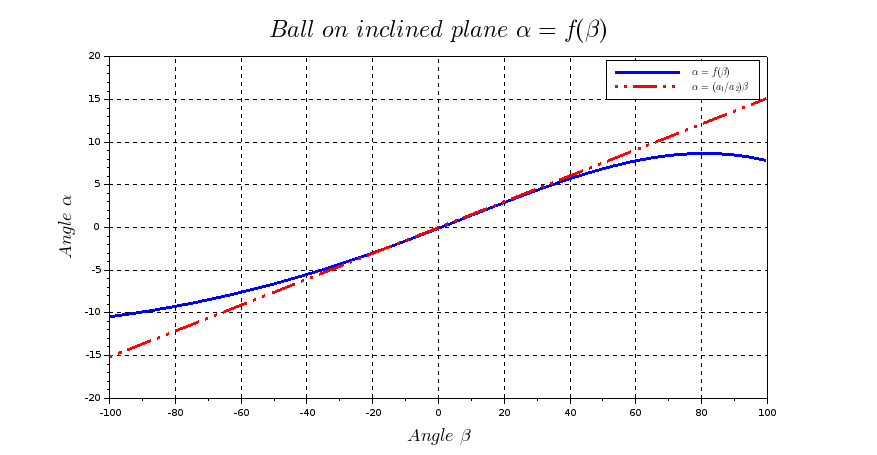
\includegraphics[scale=0.45]{images/plot1_1.png}
		\captionof{figure}{$\beta$ von -100 Grad bis +100 Grad}
	\end{minipage}
\end{center}


\subsection{Zweite Frage}
\bfseries Ausdehnung des Bereichs von $\beta$ auf $\beta \in \pm 300$ Grad \\
\mdseries Wenn der Bereich von $\beta$ auf $\beta \in \pm300$ Grad vergrößert wird, beginnt der Graph periodisch zu schwingen. Da der Servomotor den Arm auf einer Kreisbahn bewegt wiederholen sich die Werte von $\alpha$. Diese befinden sich im Bereich zwischen $-15<\alpha<10$ Grad.\\
\begin{center}
	\begin{minipage}{\linewidth}
	\centering
	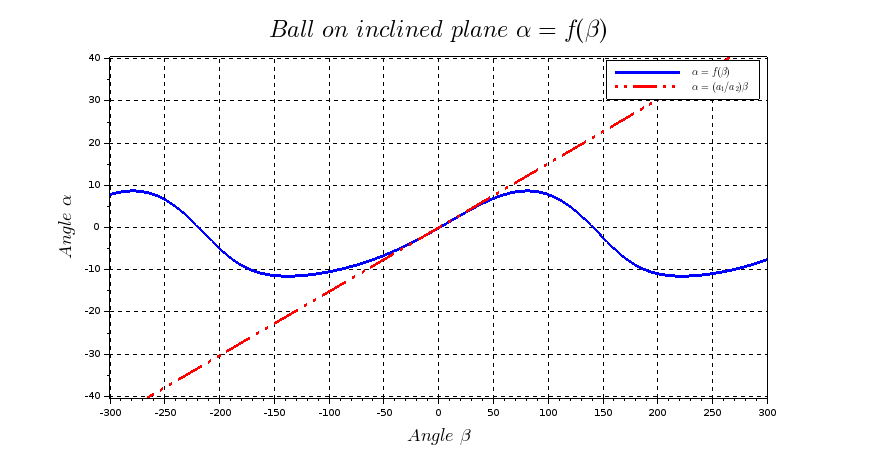
\includegraphics[scale=0.45]{images/plot2_1.png}
	\captionof{figure}{$\beta$ von -300 Grad bis +300 Grad}
	\end{minipage}
\end{center}

\subsection{Dritte Frage}
\bfseries Was geschieht, wenn man den schwarzen Arm verlängern oder verkürzen würde? \\
\mdseries Bei einem längeren Arm und sonst gleichbleibenden Parametern, hätte die Fläche bei $\beta = 0$ Grad ein Gefälle von links nach rechts. Dies könnte mit einem Offset am Motor ausgeglichen werden. Bei einer zu hohen Länge kann es passieren, dass sich die Fläche nur noch in dem Grad des Gefälles von links nach rechts variieren lässt, die Gegenrichtung also nicht mehr erreicht werden kann. \\
Bei einem kürzeren Arm wäre die Fläche bei $\beta = 0$ Grad auch nicht in der Waage. Es gäbe ein Gefälle von rechts nach links, dass auch wieder durch ein Offset am Motor ausgeglichen werden könnte. Würde der Arm eine bestimmte Kürze unterschreiten, kann es passieren, dass keine Drehung des Motors mehr möglich ist, da er hängen bleibt. \\
Die Länge des Arms sollte so gewählt sein, dass die Fläche bei $\beta = 0$ Grad in der Waage ist.